\documentclass{article}
\usepackage{graphicx}
\usepackage{amsmath}
\usepackage{array}
\usepackage[font=small, labelfont={sf,bf}, margin=1cm]{caption}
\usepackage{tabularx}
\usepackage{amssymb}
\usepackage{esint}


\date{Due: Nov 20 Edit: \today}
\title{NPRE 321 HW 6}
\author{James Liu}

\begin{document}
\maketitle
\begin{itemize}
    \item [1.]
    \begin{itemize}
        \item [a)] \
        \begin{figure}[h]
            \centering
            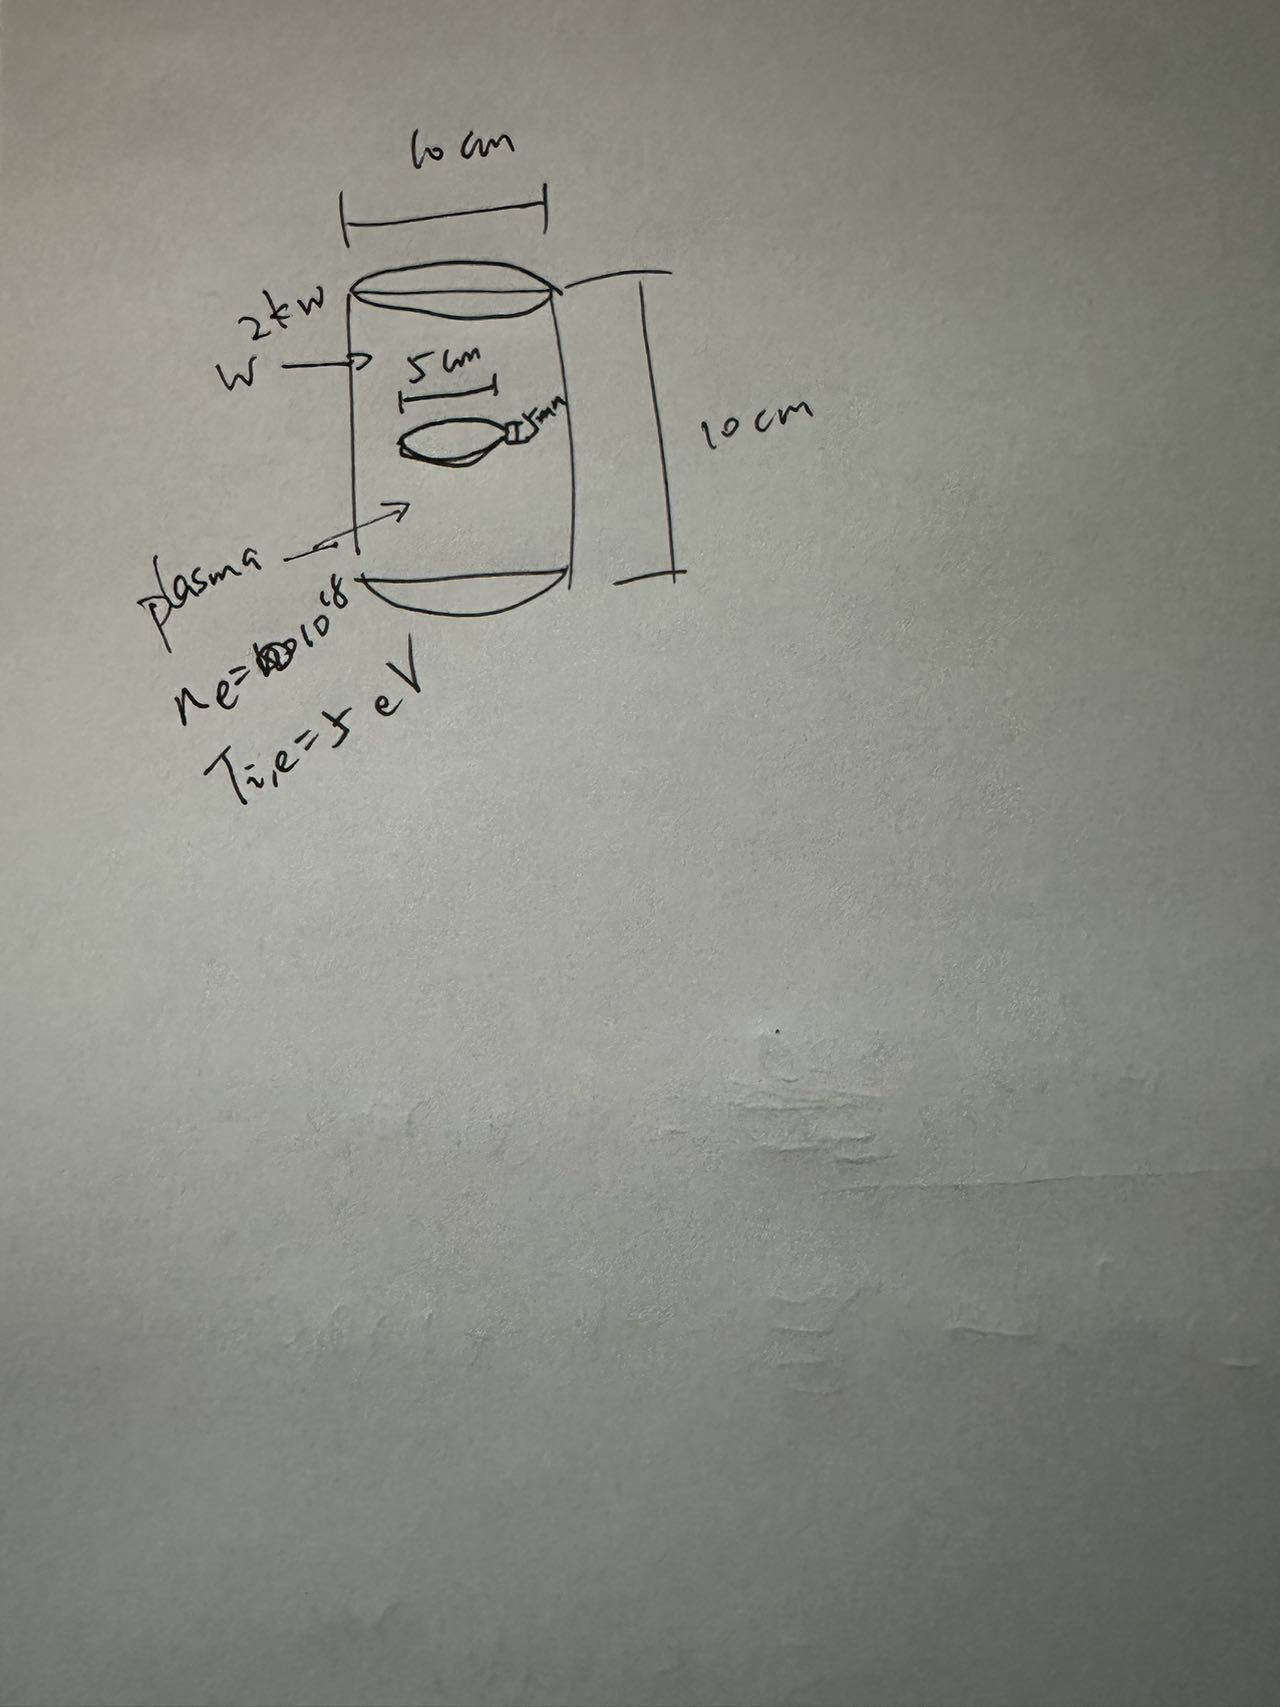
\includegraphics[scale = 0.2]{figure/npre321_HW6_fig1.jpeg}
        \end{figure}
        \item [b)]
        \begin{align*}
            S &= \pi d h + 2(\frac{1}{2}d)^2\pi\\
            &=0.01\pi+0.005\pi\\
            &=0.015\pi \text{ m}^2\\
            \Gamma_q &=\frac{P}{S}\\
            &=\frac{2000}{0.015\pi}\\
            &=42441.3 \text{ W/m}^2
        \end{align*}
        \item [c)]
        \begin{align*}
            S_{Cu}&=\pi d h + 2(\frac{1}{2}d)^2\pi\\
            &=0.00025\pi+0.00125\pi\\
            &=0.0015\pi\\
            V &= 2(\frac{1}{2}d)^2\pi \times h\\
            &=1.963495\times 10^{-5} \text{ m}^3\\
            Q &= \Gamma_q t S\\
            &=42441.3\times (5\times 60)\times 0.0015\pi\\
            &=6\times 10^4 \text{ J}\\
            Q&=mC_p\Delta T\\
            \Delta T &= \frac{Q}{mC_p}\\
            &=\frac{Q}{\rho V C_p}\\
            &=\frac{6\times 10^4}{8.9\times 10^3\times 1.963495\times 10^{-5}\times 390}\\
            &=880.373 \text{ K}
        \end{align*}
        \item [d)]
        Since for 5 min, the copper sheet is heated up 880 kelvine. Therefore, it will be mealting down if running on higher power or longer  time. However, as we covered in Practicum 2, we chould run coolants like water to cool down the copper sheet.
        \item [e)]
        \begin{align*}
            \Gamma &=\bar{n}\bar{v}\\
            &=\bar{n}\times \sqrt{\frac{8T_i}{\pi m_i}}\\
            &=10^{18}\times \sqrt{\frac{8\times 5\times 1.602\times 10^{-19}}{\pi\times  34.948 \times 1.66\times 10^{-27}}}\\
            &=5.929\times 10^{21} \text{ m}^{-2}\text{s}^{-1}
        \end{align*}
        \item [f)]
        \begin{align*}
            \dot{n}&=\Gamma \times t\\
            &=5.929\times 10^{21}\times 60^2\\
            &=2.135\times 10^{25} \text{ m}^{-2}
        \end{align*}
        \item [g)]
        \begin{align*}
            E_{i} &= 6\times T_i \\
            &=30 \text{ eV} > 3.5 \text{ eV}
        \end{align*}
        Thus, yes, the ion would be able to suppter copper away.
        \begin{align*}
            Y(100)&=0.5\\
            Y(3.5)&=0\\
            \text{Assume linear locally}\\
            Y(30)&=0.1373\\
            S_{Cu}&=\pi d h + 2(\frac{1}{2}d)^2\pi\\
            &=0.00025\pi+0.00125\pi\\
            &=0.0015\pi\\
            \dot n &=2.135\times 10^{25}\\
            N &=S_{Cu}\cdot \dot n\\
            &=1.006\times 10^{23}\\
            N_{Cu} &= N\times Y\\
            &=1.381\times 10^{22}\\
            M_{\text{Remove,}Cu} &= N_{Cu}\times m_{Cu}\\
            &=1.381\times 10^{22}\times 63.546 \times 1.66 \times 10^{-27}\\
            &=0.001457 \text{kg}\\
            M_{\text{Target,}Cu} &=\rho V\\
            &=8.9\times 10^3 \times 1.963495\times 10^{-5} \text{ m}^3\\
            &=0.194751 \text{ kg}\\
            \frac{M_{\text{Remove,}Cu}}{M_{\text{Target,}Cu}}&=0.8337 \%
        \end{align*}
    \end{itemize} 
    \item [2.]
    \begin{itemize}
        \item [a)]
        \begin{align*}
            D+D\rightarrow T+p\\
            D+D\rightarrow {}^3He + n
        \end{align*}
        \item [b)]
        \begin{align*}
            E&=mc^2\\
            &=2(m_{D})c^2\\
            &=2\times (2.014102\times 1.66\times 10^{-27}) (3\times 10^8)^2\\
            &=6.01814\times 10^{-10} \text{ J}
        \end{align*}
        \begin{itemize}
            \item [\(D+D\rightarrow T+p\)]
            \begin{align*}
                E &=(3.016049+1.00727647)\times 1.66\times 10^{-27}\times (3\times 10^8)^2\\
                &=6.01085\times 10^{-10} \text{ J}\\
                \Delta E &=6.01814\times 10^{-10} \text{ J}-6.01085\times 10^{-10} \text{ J}\\
                &=7.288\times 10^{-13} \text{ J}\\
                &=4.5495\times 10^6 \text{ eV}
            \end{align*}
            \item [\(D+D\rightarrow {}^3He + n\)]
            \begin{align*}
                E &=(3.016029+1.008665)\times 1.66\times 10^{-27}\times (3\times 10^8)^2\\
                &=6.01289\times 10^{-10} \text{ J}\\
                \Delta E &= 6.01814\times 10^{-10} - 6.01289\times 10^{-10}\\
                &=5.24394\times 10^{-13} \text{ J}\\
                &=3.273 \times 10^6 \text{ eV}
            \end{align*}
        \end{itemize}
        \item [c)]\ 
        \begin{itemize}
            \item [\(D+D\rightarrow T+p\)]
            \begin{align*}
                \frac{T}{2D} &= \frac{3.016049}{2\times 2.014102}\\
                &=74.8733 \%\\
                \frac{p}{2D} &= \frac{1.00727647}{2\times 2.014102}\\
                &=25.0056 \%
            \end{align*}
            \item [\(D+D\rightarrow {}^3He + n\)]
            \begin{align*}
                \frac{{}^3He}{2D} &= \frac{3.016029}{2\times 2.014102}\\
                &=74.8728 \%\\
                \frac{n}{2D} &= \frac{1.00727647}{2\times 2.014102}\\
                &=25.0401  \%
            \end{align*}
        \end{itemize}
    \end{itemize}
\end{itemize}
\end{document}